\chapter{Objetivos }\label{objetivos}

En este capítulo se plantean los objetivos a cumplir con este proyecto, así como los requisitos, la metodología y el plan de trabajo que se ha seguido para alcanzarlos.

\section{Objetivos}

El objetivo principal de este trabajo es introducir la \textit{gamificación} en la plataforma Kibotics. Lo hemos articulado en los siguientes tres subobjetivos u objetivos específicos a cumplir:

\begin{itemize}
    \item Diseñar y desarrollar un nuevo juego que analice el audio en tiempo real y explorar la posibilidad de añadir bandas sonoras a los ejercicios actuales. 

    \item Diseñar y desarrollar un nuevo ejercicio sobre una aspiradora robótica que tiene que limpiar una habitación.

    \item Diseñar y desarrollar un nuevo ejercicio sobre un robot que juega al pañuelo, recorriendo una línea, recogiendo una lata que ejerce de pañuelo y regresando con ella al lugar de partida.
    
\end{itemize}

Para los tres ejercicios se desarrollará la infraestructura necesaria, modelos nuevos de robots, escenarios en el simulador, evaluadores automáticos, soluciones de referencia y se integrarán en la plataforma web de robótica eduactiva Kibotics.
    


\newpage

\section{Requisitos}
Para cumplir con los objetivos citados anteriormente debemos tener en cuenta además los siguientes  requisitos: 
\begin{itemize}
    \item Los robots y juegos desarrollados deben ser compatibles con la versión actual v.2.8 o superior de Kibotics.
    \item No se debe requerir de instalaciones adicionales. Todo debe correr en el navegador web del cliente. 
    \item Uso de software de simulación Websim y A-Frame.
\end{itemize}

 
\section{Metodología}

La metodología que se ha seguido para la realización de este trabajo es la basada en el modelo de desarrollo software iterativo y creciente (Figura 2.1) \cite{modeloiter}.
Este modelo consiste en entregar a los usuarios y al equipo de desarrolladores de Kibotics una versión disponible lo antes posible y en continua actualización. En cada iteración se van solventando pequeños errores y mejoras que convergen en la versión final del proyecto.

\begin{figure}[H]
    \centering
    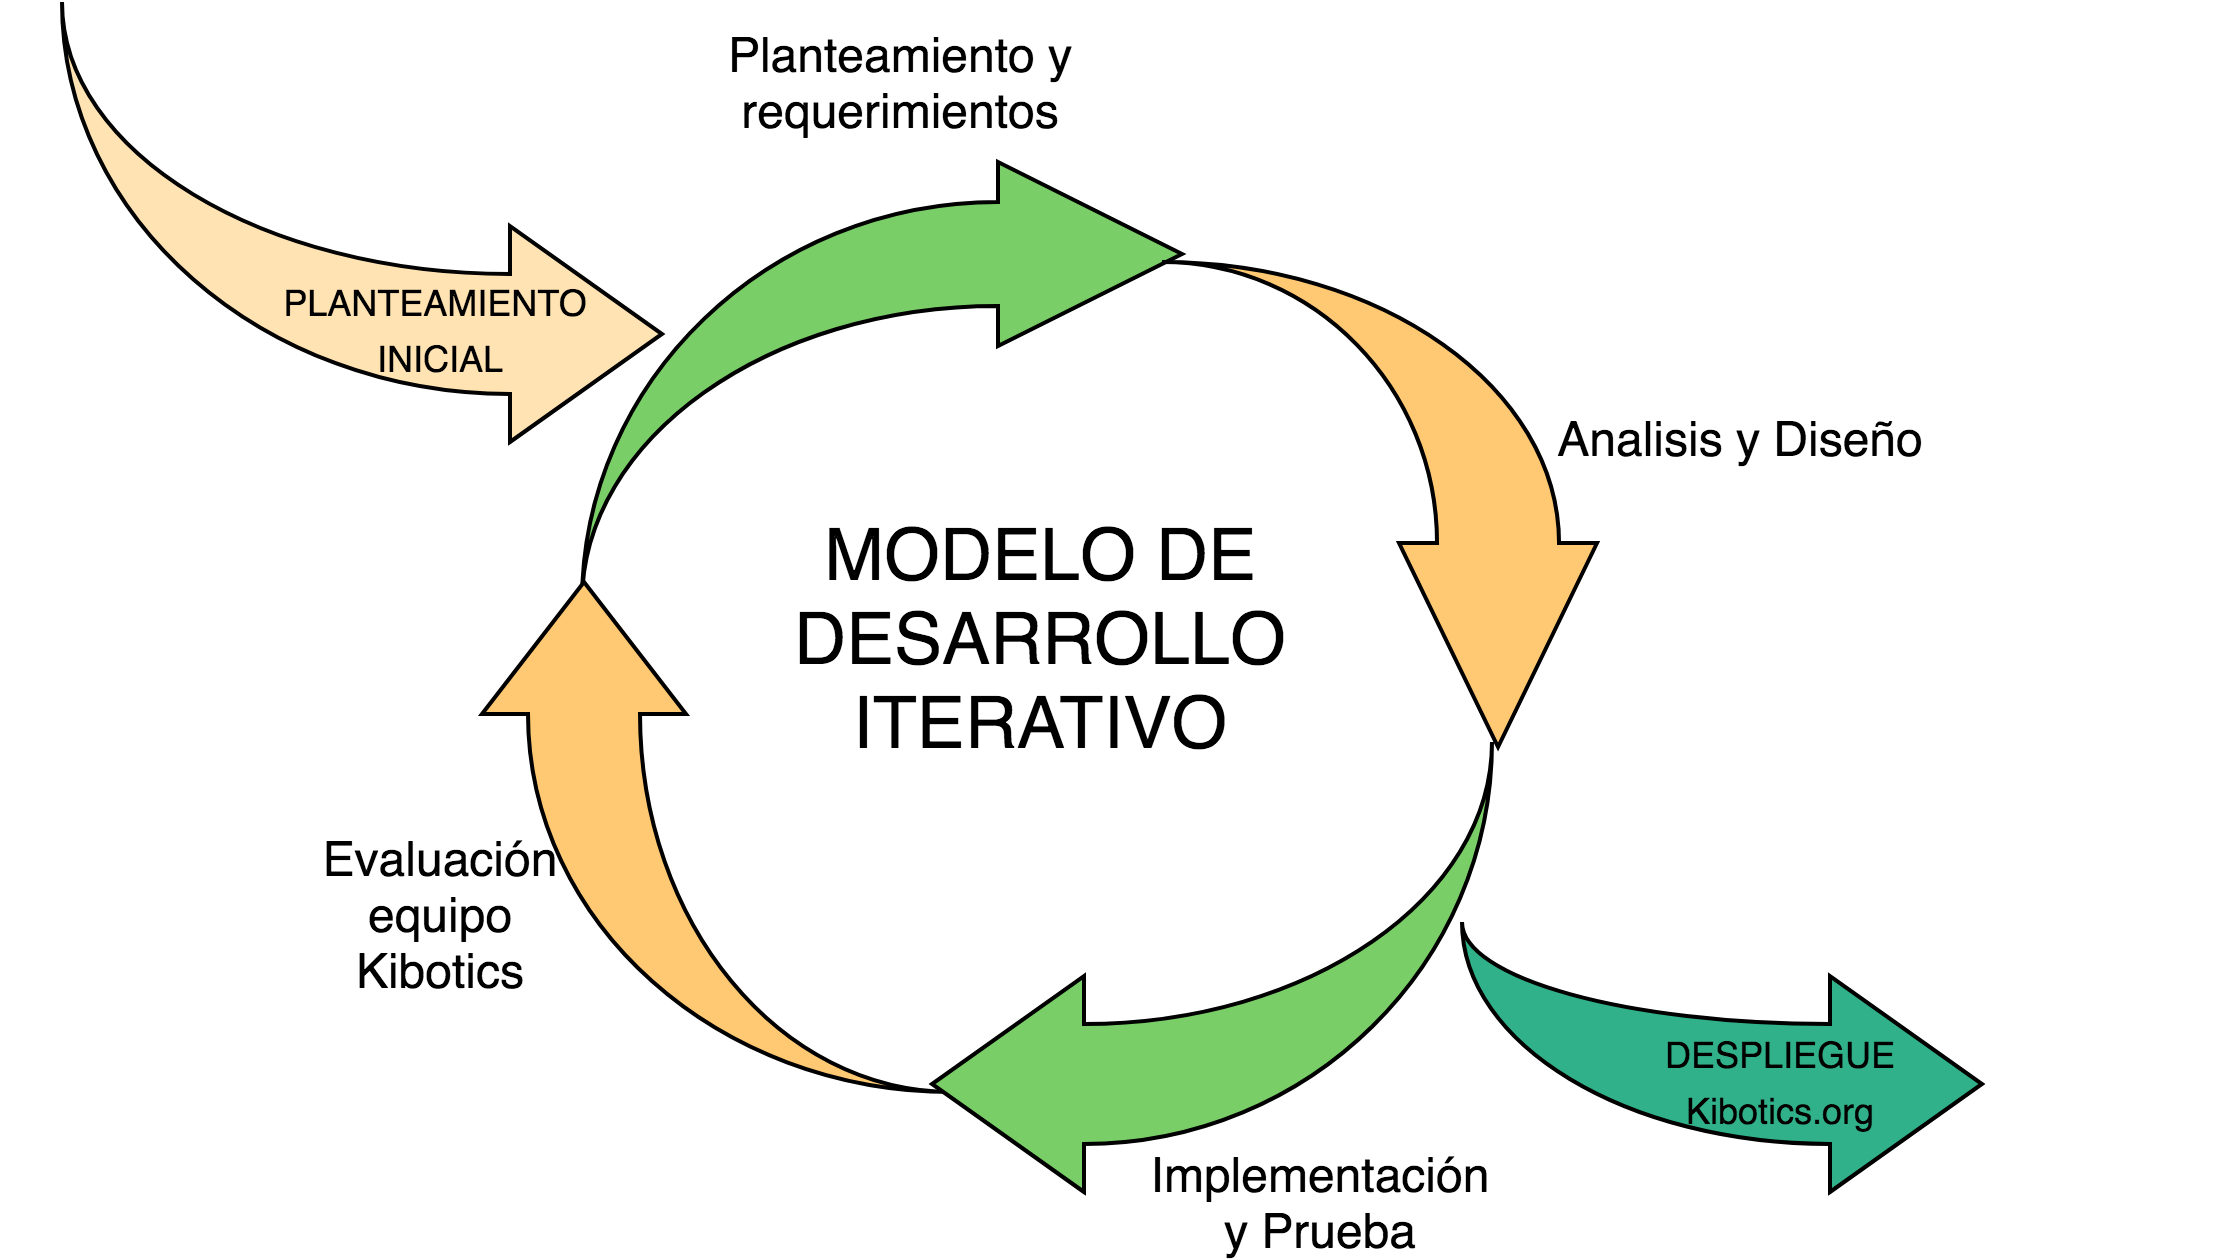
\includegraphics[width=0.6\columnwidth]{chapters/images/metodologiaiterativa.png}
    \caption{Modelo iterativo}
    \label{fig:my_label}
\end{figure}


El código desarrollado y las mejoras se han integrado progresivamente en el código fuente oficial de Kibotics en GitHub \footnote{https://github.com/} mediante su flujo de trabajo  incidencia (\textit{issue}), rama (\textit{branch}) y parche (\textit{pullresquest}). De esta forma la plataforma oficial está siempre actualizada con los últimos cambios añadidos y verificados por el equipo de desarrolladores.

Para llevar acabo esta metodología se establecieron reuniones semanales con el tutor para la orientación de este trabajo fin de grado. A lo largo del proyecto se ha mantenido la comunicación con el tutor y el equipo de Kibotics a través de la plataforma Slack \footnote{https://slack.com/}. 



Además se ha creado y mantenido  una página web tipo blog para llevar un seguimiento de las tareas realizadas y los objetivos semanales. \footnote{https://roboticslaburjc.github.io/2020-tfg-marta-quintana/}

\begin{figure}[H]
    \centering
    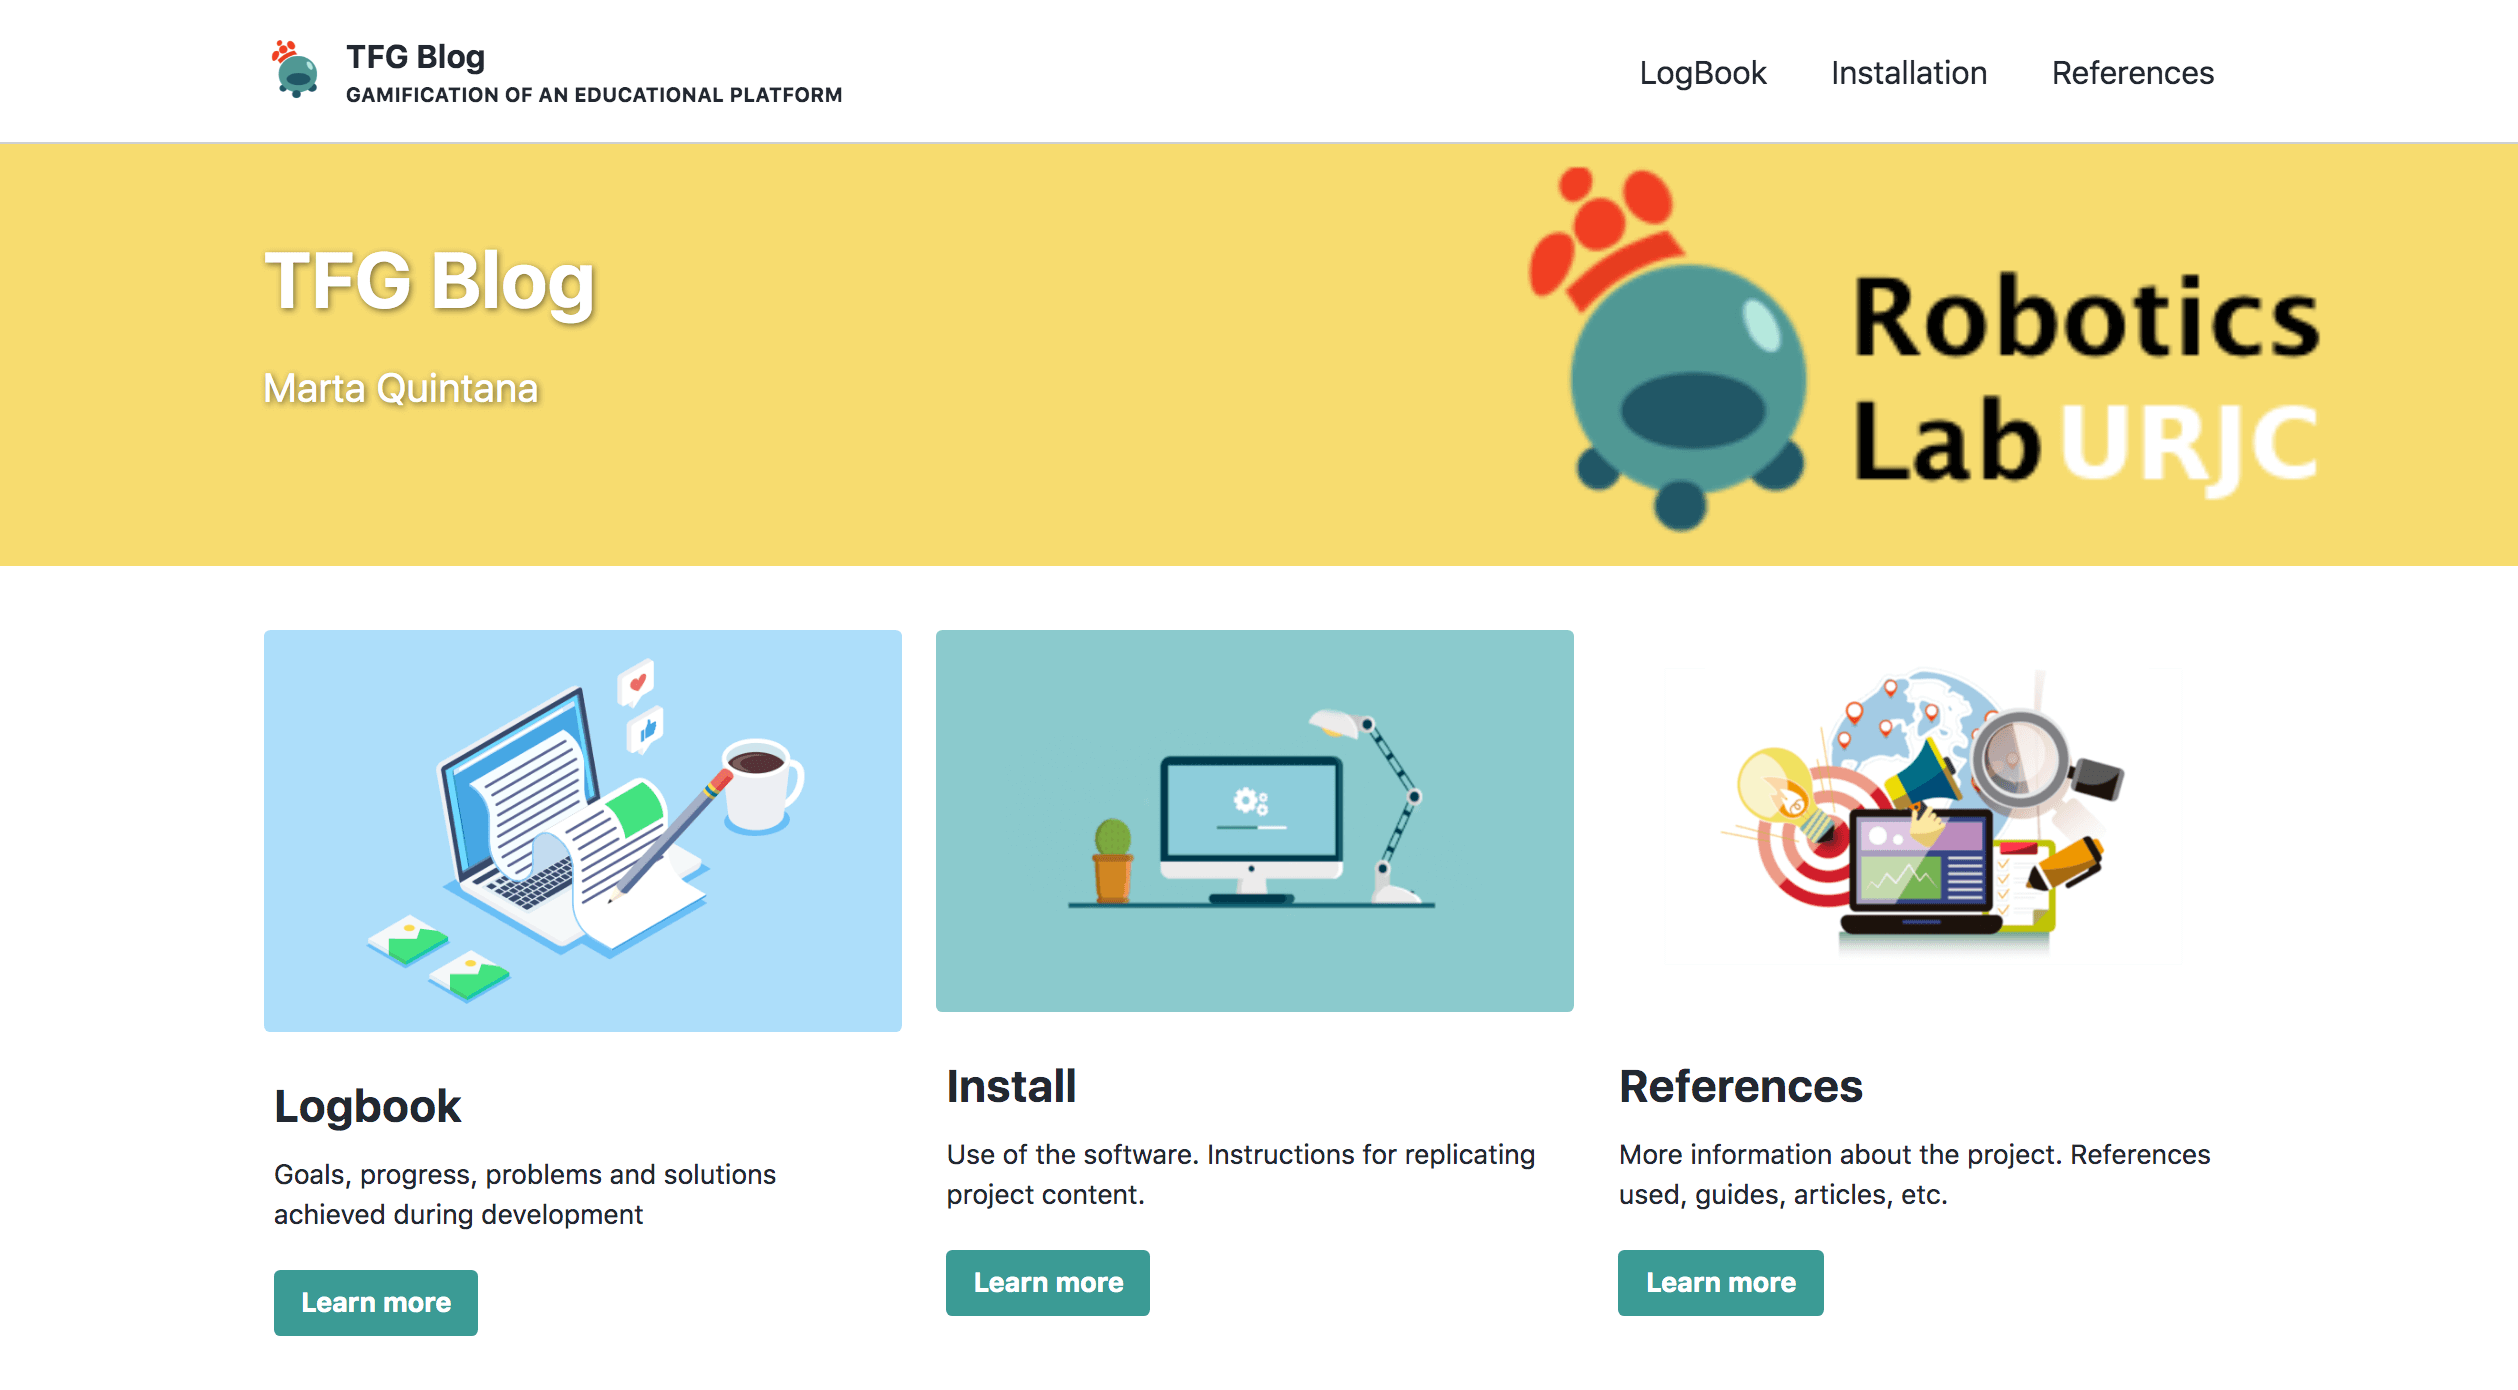
\includegraphics[width=0.6\linewidth]{chapters/images/webtfg.png}
    \caption{Página web de este TFG}
    \label{fig:my_label}
\end{figure}

\section{Plan de Trabajo}
El plan de trabajo seguido durante este proyecto se puede dividir en las siguientes etapas:


\begin{itemize}
    \item \textbf{Aterrizaje en Kibotics y repaso de tecnologías web}: Toma de contacto con Kibotics y repaso de HTML5, JavaScript, Django y otras tecnologías que se utilizan en la plataforma.
    
    \item \textbf{Estudio Web Audio API y Tensor FlowJS}: Realización de ejercicios y tutoriales de distintas herramientas para introducir sonido y reconocimiento de audio en Kibotics.
   
    \item \textbf{Diseño Teleoperador Acústico con Teachable Machine}: Creación de un teleoperador acústico con reconocimiento de audio. 

    \item \textbf{Prototipo de aspiradora robótica}: Diseño y creación de modelos del nuevo ejercicio.
    \item \textbf{Diseño ejercicio aspiradora robótica confeti}: Desarrollo de una aspiradora robótica simulada, un nuevo actuador de absorción y piezas de confeti que puedan ser absorbidas por la aspiradora.
    
    \item \textbf{Prototipo de un robot Mbot con Pinza basado en A-Frame}: Estudio de un prototipo en A-Frame nativo para el estudio de las físicas y mallas de colisión. 
    \item \textbf{Preparación del ejercicio del pañuelo}: Creación e implementación del ejercicio, desarrollo del circuito, una lata y un Mbot con Pinza realizados con Blender y JavaScript, para ofrecernos físicas más realistas.

\end{itemize}

